
During the requirement analysis of the challenge, the general model federation approach remains the foundation of our reflections and modeling intentions. 

First, the federation approach is mainly based on modeling relationships among several models, independently of abstraction levels and model architectures.
The next step in our approach, we try to take into account the reusability of the relationships by identifying the meaning, or semantics, associated with each relationship, in a goal of concept reification with their behavior. The last step is to organize or structure these concepts to improve reusability and extensibility, to create VirtualModels in our Openflexo framework.     

Like any modeling approaches, these different steps could also be achieved in any order. But our goal during the challenge requirement analysis remains to lead to define a FML Virtual Models architecture as a federation of virtualmodels. As shown in figure~\ref{fig:MultilevelArchitecture}, we developped two metamodels (Base and ACME processes abstractions) instantiatied by two models (XSure and ACME processes). This follows the way the challenge is presented and this organisation allows for the possibility of easy extensions.


\begin{figure}
    \centering
    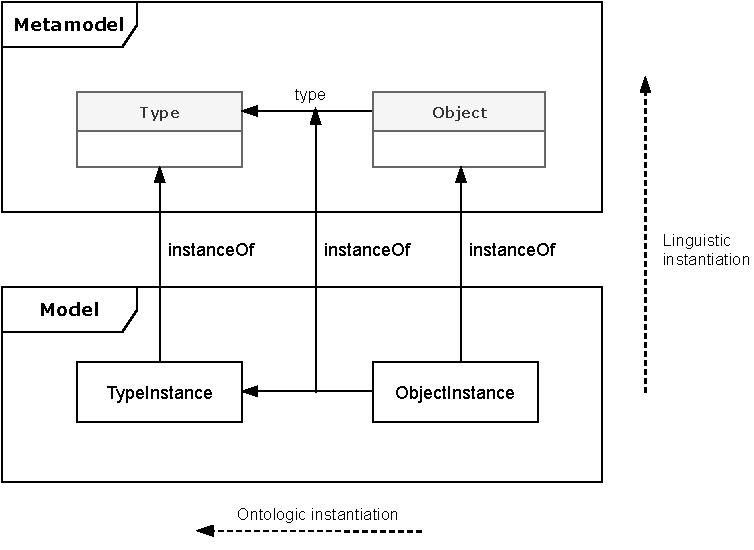
\includegraphics[width=1.0 \columnwidth]{Figures/Instantiation.pdf}
    \caption{Linguistic and ontologic instantiation}
    \label{fig:LinguisticAndOntologicInstantiation}
\end{figure}



Also as our understanding, the use case analysis leads to identify two main modeling axis (as presented in figure \ref{fig:LinguisticAndOntologicInstantiation}):
\begin{itemize}
    \item the horizontal axis is characterized as the ontological instantiation axis, in the sense that the domain type definition (ProcessType as example) is referenced by an instance definition (Process, a.e). In our base  VirtualModel, each domain type definition is referenced by its instance definition, as developed in the section \ref{sec:ProcessEnactment}

\item the vertical axis is viewed as the linguistic instantiation, relative to the use of the FML language. The VirtualModel, defined as the core definition model, generates a model founded on the instantiation mechanism of the FML Language. This mechanism is the classical Object/Instance mechanism of the object languages but without any constraint on the referenced VirtualModel. The set of resulted instances comes from several VirtualModels 
from any abstraction level as detailed in section \ref{sec:AcmeSoftwareDevelopmentProcess}


\end{itemize}



\begin{figure}
    \centering
    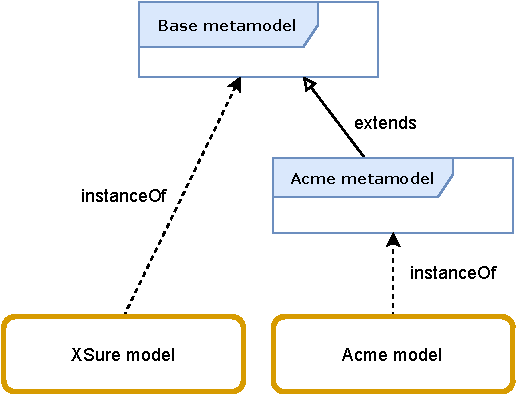
\includegraphics[width=0.7 \columnwidth]{Figures/MultilevelArchitecture.pdf}
    \caption{Multilevel architecture for the Process Challenge}
    \label{fig:MultilevelArchitecture}
\end{figure}



% il reste à décrire l'architecture générale des VirtualModels


~\\
~\\

%\emph{any disambiguations of the  case  description and assumptions made, any potentially added requirements}

\todo[inline]{quelles hypothèses supplémentaires ?}
\todo[inline]{+ architecture de la modélisation (ce qui se trouve dans le ppt), le détail se retrouvera dans la section suivante}

%Joel commence

% Sylvain
% Joel, je te propose les deux figures suivantes:


